\documentclass[a4paper]{article}

%% Language and font encodings
\usepackage[english]{babel}

\usepackage[T1]{fontenc}
\usepackage[utf8]{inputenc}

%% Sets page size and margins
\usepackage[a4paper,top=3cm,bottom=2cm,left=3cm,right=3cm,marginparwidth=3cm]{geometry}

%% Useful packages
\usepackage{amsmath}
\usepackage{graphicx}
\usepackage[colorinlistoftodos]{todonotes}
\usepackage[colorlinks=true, allcolors=blue]{hyperref}
\usepackage{subfig}
\usepackage{float}

%\usepackage{biblatex}
%\addbibresource{assign2ref.bib}
%\usepackage{csquotes}

%\setlength{\tabcolsep}{0pt}

% Write the title here
\title{Pattern Recognition\\
	Assignment 2\\
	Group No - 36 }
\author{ED13D000 Bhargava Sai Ramu\\
	CS17S008 Nitesh Methani}

\begin{document}
\maketitle
\hypersetup{linkcolor=black}
\tableofcontents


% Introduction
\section{Introduction}
We have three datasets to work with. One dataset is linearly seperable that means all the classes can be seperated using linear lines. Second dataset is Non-Linearly Seperable dataset that means we should get non linear decision boundaries between each class. Third dataset is Linearly Non Seperable dataset it means data cannot be seperated using linear lines.
\newpage



% Linearly Separable Data Plots
\section{Linearly Separable Data-set}
\begin{figure}[H]
	\hspace*{-2cm}\begin{tabular}{cc}
		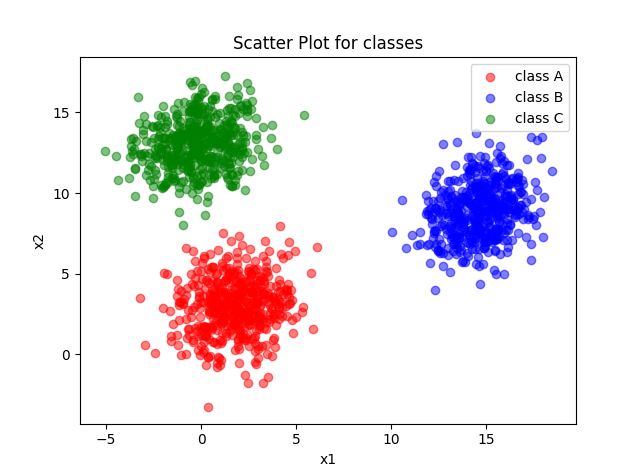
\includegraphics[width=70mm]{./dataset1/scatter.png} &   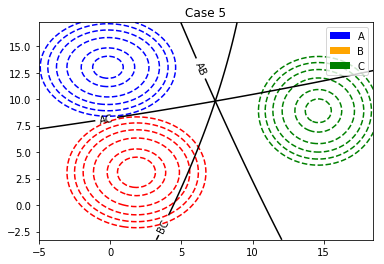
\includegraphics[width=70mm]{./dataset1/contour.png} \\
		(a) Scatter Plot for each class & (b) Constant Density Curves and Decision Boundaries\\[4pt]
		
		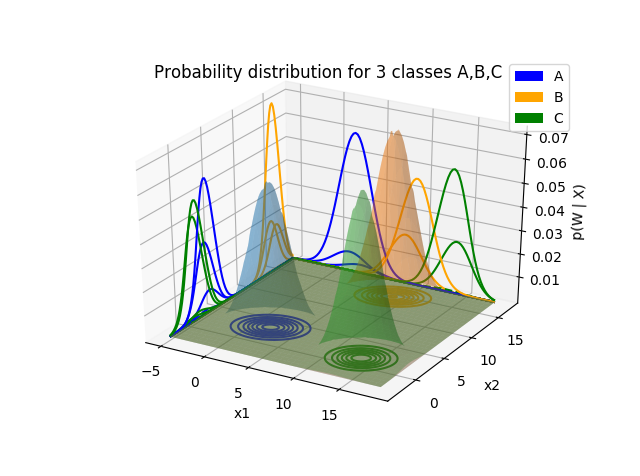
\includegraphics[width=70mm]{./dataset1/PDF.png} &   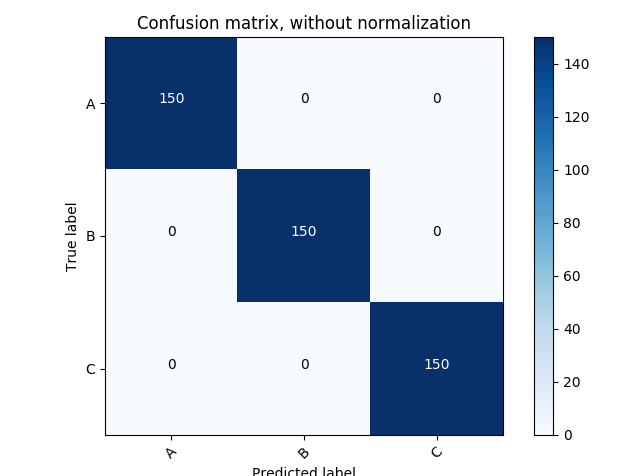
\includegraphics[width=70mm]{./dataset1/confusionMatrix.png} \\
		(c) Gaussian Distributions for each class and feature & (d) Confusion Matrix \\[4pt]
		
		%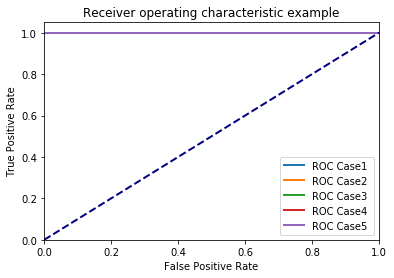
\includegraphics[width=70mm]{./dataset1/roc.png} &   %\includegraphics[width=70mm]{} \\
		%(e) ROC Curve & (f) DET Curve \\[4pt]		
		
		
		
		% To plot 5 images i 3x2 table
		\multicolumn{2}{c}{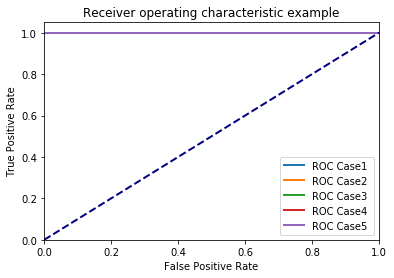
\includegraphics[width=70mm]{./dataset1/roc.png} }\\
		\multicolumn{2}{c}{(e) ROC Curve}
		
	\end{tabular}\hspace*{-1cm}
	\caption{Summary of Linearly Separable Dataset}
\end{figure}

% Non-Linearly Separable Data Plots
\section{Non-Linearly Separable Data-set}
\begin{figure}[H]
	\hspace*{-2cm}\begin{tabular}{cc}
		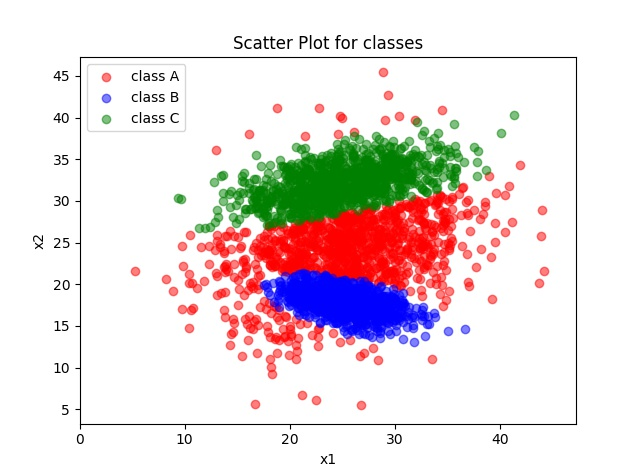
\includegraphics[width=70mm]{./dataset2/scatter.jpeg} &   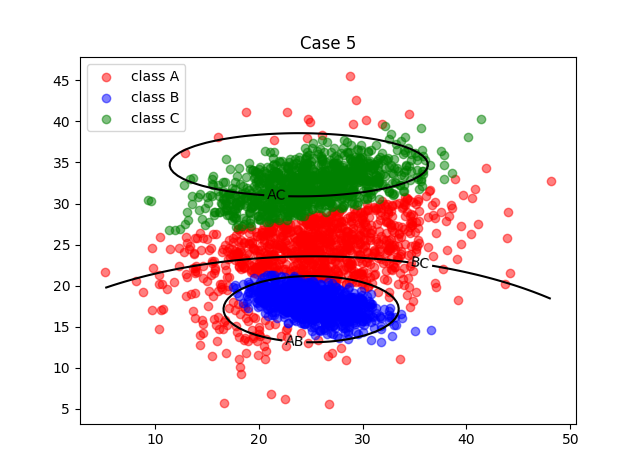
\includegraphics[width=70mm]{./dataset2/decisio.png} \\
		(a) Scatter Plot for each class & (b) Constant Density Curves and Decision Boundaries\\[4pt]
		
		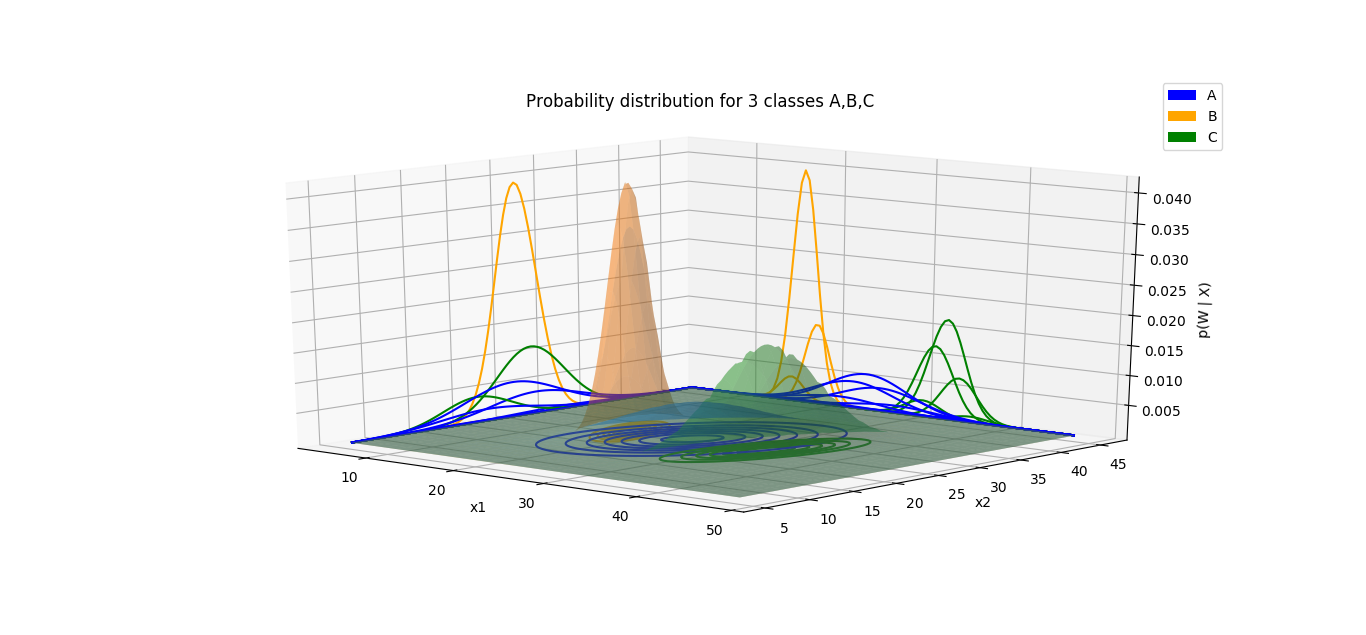
\includegraphics[width=70mm]{./dataset2/PDF.png} &   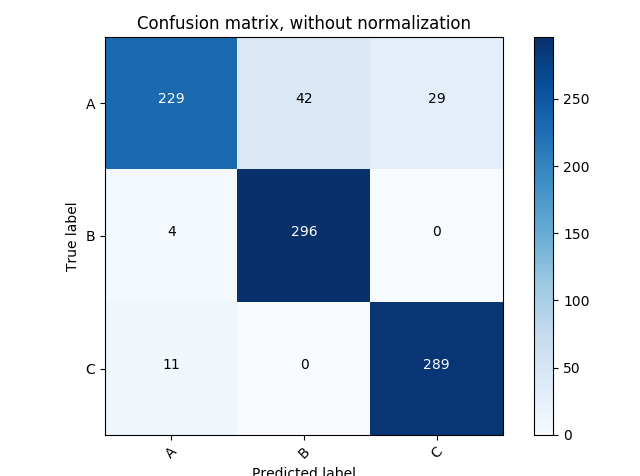
\includegraphics[width=70mm]{./dataset2/confusionMatrix.png} \\
		(c) Gaussian Distributions for each class and feature & (d) Confusion Matrix \\[4pt]
		
		%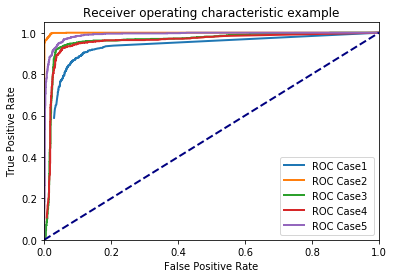
\includegraphics[width=70mm]{./dataset2/roc.png} &   %\includegraphics[width=70mm]{} \\
		%(e) ROC Curve & (f) DET Curve \\[4pt]		
		
		
		% To plot 5 images i 3x2 table
		\multicolumn{2}{c}{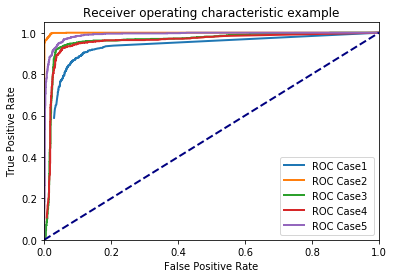
\includegraphics[width=70mm]{./dataset2/roc.png} }\\
		\multicolumn{2}{c}{(e) ROC Curve}
		
	\end{tabular}\hspace*{-1cm}
	\caption{Summary of Linearly Non Separable Dataset}
\end{figure}

% Linearly Non-Separable Data Plots
\section{Linearly Non-Separable Data-set}
\begin{figure}[H]
	\hspace*{-2cm}\begin{tabular}{cc}
		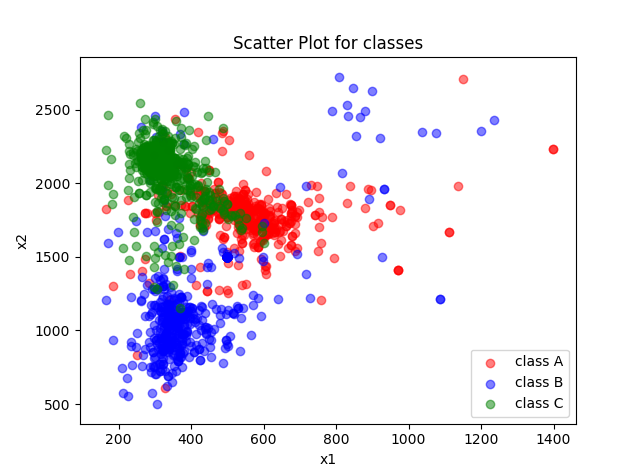
\includegraphics[width=70mm]{./dataset3/scatter.png} &   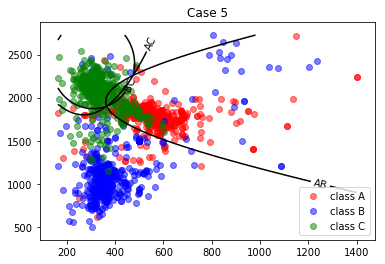
\includegraphics[width=70mm]{./dataset3/decisio.png} \\
		(a) Scatter Plot for each class & (b) Constant Density Curves and Decision Boundaries\\[4pt]
		
		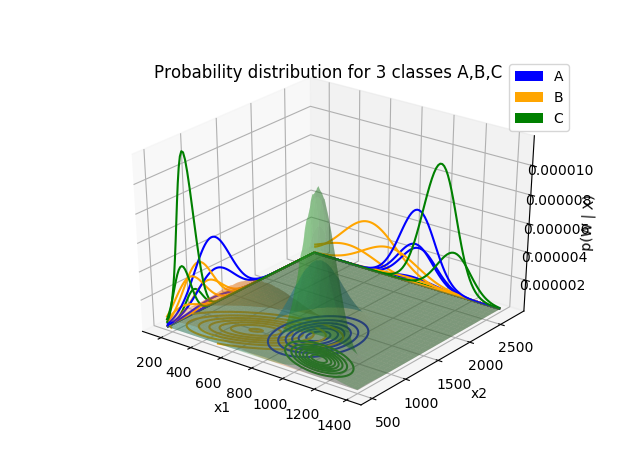
\includegraphics[width=70mm]{./dataset3/PDF.png} &   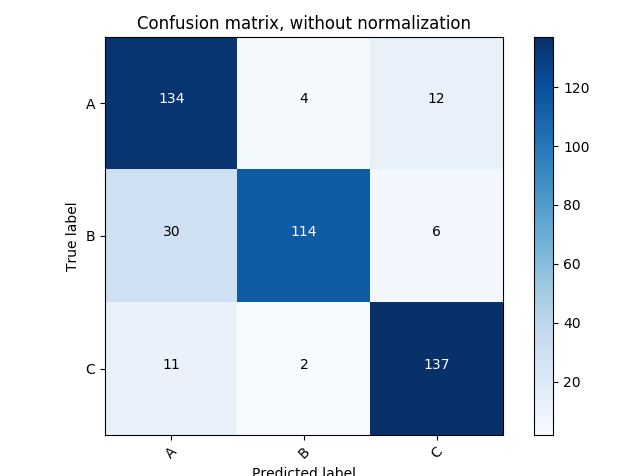
\includegraphics[width=70mm]{./dataset3/confusionMatrix.png} \\
		(c) Gaussian Distributions for each class and feature & (d) Confusion Matrix \\[4pt]
		
		%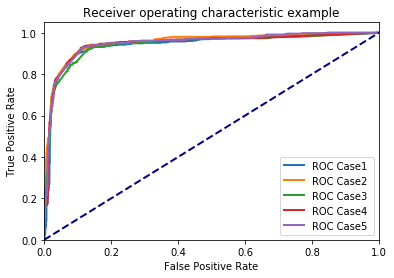
\includegraphics[width=70mm]{./dataset3/roc.png} 
		%(e) ROC Curve \\[4pt]		
		
		
		
		% To plot 5 images i 3x2 table
		\multicolumn{2}{c}{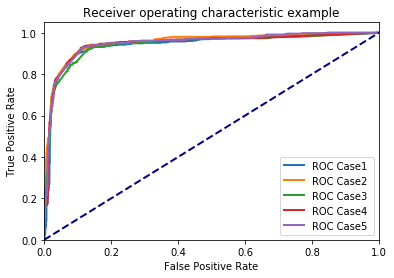
\includegraphics[width=70mm]{./dataset3/roc.png} }\\
		\multicolumn{2}{c}{(e) ROC Curve}
		
	\end{tabular}\hspace*{-1cm}
	\caption{Summary of Non Linearly Separable Dataset}
\end{figure}
\newpage
\section{Observations:}

1) If the constant density curves are circles that means the covariance matrix for all the classes is same which is nothing but our case 1 and case 4.\\
2) Eigen vectors are perpendicular to the lines joining the means of each distribution in case 1 and case 4.\\
3) Whereas for other cases when covariance matrix for all the classes is different, the constant density curves are ellipsoids.\\
4) Eigen vectors of these hyper-ellipsoids shows the distribution of the data points along the principal axes of the ellipsoid.\\
5) If I move along the major axis or minor axis density goes on reducing or increasing depending on the case.\\
6) The decision boundaries are not perpendicular in case 2 and case 5.\\
7) The decision boundaries are not perpendicular in case 1.\\
8) The nature of the ROC and DET curves that we got match with the theory we studied in class.\\
9) The confusion matrix also justify the metrics.\\
10) For real data, all the points are not properly classified since decision boundaries are not ale to make distinction between all the three classes so accuracy and other metrics are not upto the mark in this case.\\
11) For linearly separable dataset and non-linearly separable dataset the accuracy is pretty high.\\



%\section{References}


%\printbibliography
\end{document}